
% part 3

\section{Наш первый взгляд на Twisted\label{sec:part3}}

\subsection{Ничего не делать - путь Twisted}

На данный момент мы нацелены на улучшение кода  
асинхронного поэтического клиента,  
используя Twisted. Cначала давайте напишем 
несколько простых Twisted программ,  
чтобы осознать cуть вещей. Как было упомянуто в главе 2,  
примеры были отлажены с использованием Twisted 8.2.0. API 
в Twisted меняется, но основные API, которые мы собираемся использовать 
меняются медленно, поэтому примеры 
будут актуальны и для cледующих релизов. Если у вас не 
установлен Twisted, вы можете получить его 
\href{http://twistedmatrix.com/trac/wiki/Downloads}{здесь}.


Самая простая Twisted программа представлена ниже. Код можно 
найти в директории с примерами в файле    
\href{http://github.com/jdavisp3/twisted-intro/blob/master/basic-twisted/simple.py}{basic-twisted/simple.py}. 

\begin{scriptsize}\begin{verbatim}
from twisted.internet import reactor
reactor.run()
\end{verbatim}\end{scriptsize}

Пример запускается следующим образом:

\begin{scriptsize}\begin{verbatim}
python basic-twisted/simple.py
\end{verbatim}\end{scriptsize}

В предыдущей главе мы выяснили, что Twisted - реализация шаблона проектирования 
\href{http://en.wikipedia.org/wiki/Reactor\_pattern}{Reactor}, 
таким образом Twisted содержит объект, который представляет reactor или 
event loop, который является ядром любой Twisted программы. Первая строка 
нашей программы импортирует объект reactor, чтобы его можно было   
использовать, вторая строка запускает цикл реактора. 


Программа выше ничего не делает. Остановить ее можно, 
нажав Ctrl-C, иначе она будет вечно ничего не делать. 
Обычно в цикле мониторятся на ввод-вывод какие-нибудь 
файловые дескрипторы (например, соединенные с поэтическим 
сервером). Позже, мы сделаем это, но сейчас 
цикл реактора простаивает. Заметьте, что это не 
\href{http://en.wikipedia.org/wiki/Busy\_waiting}{busy loop}, 
который реально выполняет цикл. Если посмотреть 
на загруженность процесса, то не будет видно никаких 
всплесков. Фактически, наша программа совсем не использует 
процессор. Вместо этого reactor простаивает наверху 
цикла рисунка \ref{fig:reactor-1}, ожидая события, которое 
никогда не произойдет (в реальности, ожидая возврата 
вызова select без файловых дескрипторов).


Сделаем несколько выводов:

\begin{enumerate}
\item Цикл реактора в Twisted запускается явно вызовом reactor.run().

\item Цикл реактора запускается в том же треде, где он 
был запущен. В примере выше, он был запущен в единственном main треде. 

\item После запуска цикл бесконечно продолжается.

\item Если нет задач, цикл реактора не потребляет процессор.

\item reactor явно не создается, он просто импортируется.
\end{enumerate}


Последний пункт стоит обсудить. Twisted reactor -  
\href{http://en.wikipedia.org/wiki/Singleton\_pattern}{Singleton}. 
Существует только один объект reactor, и он создается неявно при импорте. 
Если открыть модуль reactor в пакете twisted.internet, то кода там будет 
очень мало. Реальная реализация находится в другом файле:
\newline (\href{http://twistedmatrix.com/trac/browser/tags/releases/twisted-8.2.0/twisted/internet/selectreactor.py}{twisted.internet.selectreactor.py}).


В Twisted есть много различных реализаций реактора. Как было упомянуто 
в главе 2, вызов select'а - это один из способов ожидания событий на 
файловых дескрипторах. По умолчанию, Twisted использует select, 
но Twisted также включает и другие типы реакторов. Например, 
\href{http://twistedmatrix.com/trac/browser/tags/releases/twisted-8.2.0/twisted/internet/pollreactor.py}{twisted.internet.pollreactor}, который использует системный вызов 
\href{http://www.makelinux.net/ldd3/chp-6-sect-3.shtml}{poll} вместо 
select.


Для использования другого реактора нужно установить его до 
импортирования twisted.internet.reactor. Вот так можно 
установить pollreactor:

\begin{scriptsize}\begin{verbatim}
from twisted.internet import pollreactor
pollreactor.install()
\end{verbatim}\end{scriptsize}


Если проимпортировать twisted.internet.reactor без 
установки определенной реализации реактора, то 
Twisted установит reactor на основе select. 
По этой причине не импортируйте reactor в начале 
модулей, чтобы избежать случайной установки 
реактора по умолчанию, вместо этого импортируйте 
в том же месте, где собираетесь использовать.


Стоит заметить, что на момент написания статьи, Twisted двигается в 
сторону архитектуры, которая позволила бы использовать 
несколько реакторов одновременно. В такой схеме объект 
reactor мог бы подставляться как ссылка, а не как объект,  
импортированный из модуля.


Сейчас можно переписать нашу первую Twisted программу, 
используя pollreactor, которую можно найти в 
\href{http://github.com/jdavisp3/twisted-intro/blob/master/basic-twisted/simple-poll.py}{basic-twisted/simple-poll.py}:

\begin{scriptsize}\begin{verbatim}
from twisted.internet import pollreactor
pollreactor.install()

from twisted.internet import reactor
reactor.run()
\end{verbatim}\end{scriptsize}

Таким образом, мы имеем poll цикл, который ничего не делает, вместо 
ничего не делающего select цикла. 


Далее мы везде будем придерживаться реактора по умолчанию. Все 
реакторы Twisted делают одно и тоже.


\subsection{Привет, Twisted}

Давайте сделаем программу Twisted, которая что-нибудь делает. 
Например, программу, печатающую сообщение в окне терминала, 
после запуска цикла реактора:

\begin{scriptsize}\begin{verbatim}
def hello():
    print 'Hello from the reactor loop!'
    print 'Lately I feel like I\'m stuck in a rut.'

from twisted.internet import reactor

reactor.callWhenRunning(hello)

print 'Starting the reactor.'
reactor.run()
\end{verbatim}\end{scriptsize}

Код программы находится в 
\href{http://github.com/jdavisp3/twisted-intro/blob/master/basic-twisted/hello.py}{basic-twisted/hello.py}. 
После запуска получится следующий вывод:

\begin{scriptsize}\begin{verbatim}
Starting the reactor.
Hello from the reactor loop!
Lately I feel like I'm stuck in a rut.
\end{verbatim}\end{scriptsize}

Программу выше все еще надо завершать самостоятельно, 
поскольку она бесконечно выполняется после того, как напечатает 
строки выше.


Заметьте, что функция hello вызывается после того, как reactor 
начал выполняться. Это означает, что функция вызывается 
реактором, то есть код Twisted должен вызывать эту функцию. 
Это происходит благодаря вызову метода реактора callWhenRunning с 
ссылкой на функцию, которую должен вызвать Twisted. И, конечно же, 
мы должны вызвать callWhenRunning до того, как мы запустим 
reactor.


Термин callback означает ссылку на функцию (например, на 
функцию hello), которую мы 
передаем Twisted (или какой-то другой системе), 
которую Twisted будет использовать для того, чтобы "вызывать"  
в определенное время. В примере выше такой вызов происходит 
сразу же после того, как reactor запустится. Поскольку 
цикл в Twisted отделен от нашего кода, большинство 
взаимодействий между ядром реактора и логикой программы 
будет осуществляться через callback'и, которые 
мы передали Twisted, используя различные API.   


Мы можем увидеть то, как Twisted вызывает наш код, 
используя следующую программу:

\begin{scriptsize}\begin{verbatim}
import traceback

def stack():
    print 'The python stack:'
    traceback.print_stack()

from twisted.internet import reactor
reactor.callWhenRunning(stack)
reactor.run()
\end{verbatim}\end{scriptsize}


Код находится в 
\href{http://github.com/jdavisp3/twisted-intro/blob/master/basic-twisted/stack.py}{basic-twisted/stack.py}, 
и он напечатает что-то вроде этого:

\begin{scriptsize}\begin{verbatim}
The python stack:
...
  reactor.run() <-- This is where we called the reactor
...
...  <-- A bunch of Twisted function calls
...
  traceback.print_stack() <-- The second line in the stack function
\end{verbatim}\end{scriptsize}


Не обращайте внимание на все строки, просто 
осознайте взаимосвязь между вызовом  reactor.run() и 
нашим callback'ом. 


\subsection{Кто использует callback'и?}

Twisted не единственная система, которая использует callback'и. 
Более старые асинхронные Python системы 
\href{http://www.nightmare.com/medusa/}{Medusa} и 
\href{http://docs.python.org/library/asyncore.html#module-asyncore}{asyncore} 
также их используют. Помимо этого, многие GUI библиотеки, в том числе    
\href{http://gtk.org/}{GTK} и \href{http://qt.nokia.com/}{QT}, 
основаны на цикле реактора.


Отметим некоторые вещи:

\begin{enumerate}
\item Шаблон проектирования reactor однопоточный.
\item Реактивная система, подобная Twisted, реализует цикл 
реактора так, что наш код не должен его реализовывать.
\item Наш код должен реализовывать основную логику программы. 
\item Поскольку программа выполняется в одном потоке, 
цикл реактора будет вызывать наш код.
\item reactor не может знать наперед какую часть нашего кода нужно вызвать.
\end{enumerate}

Использование callback'ов, является неотъемлемой 
частью асинхронного программирования.

\eject

Рисунок \ref{fig:reactor-callback} показывает, что случается во время 
обратного вызова:

% fig6
\begin{figure}[h]
\begin{center}
    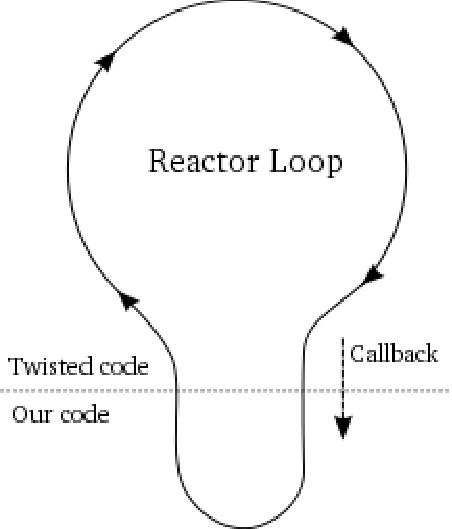
\includegraphics[width=0.5\textwidth]{images/reactor-callback.pdf}
    \caption{reactor, делающий обратный вызов\label{fig:reactor-callback}}
\end{center}
\end{figure}


Рисунок \ref{fig:reactor-callback} иллюстрирует некоторые важные особенности 
callback'ов:

\begin{enumerate}
\item Код нашего callback'а запускается в том же потоке, что и Twisted цикл.
\item Когда наши callback'и выполняются, цикл Twisted не выполняется. 
\item И наоборот.
\item Цикл реактора начинает выполняться после возврата из callback'ов.
\end{enumerate}


Во время вызова callback-функции, цикл Twisted 
блокируетяся на нашем коде. Поэтому нам следует 
убедиться, что код нашего callback'а не тратит 
время зря. То есть нам нужно избегать реализации 
блокирующего ввода-вывода в коде callback'ов. 
Иначе, использование реактора окажется бесмысленным. 
Twisted не имеет никаких специальных мер для 
предотвращения кода от блокирования, мы сами 
должны заботиться об этом. Как мы увидим позже, 
в большинстве случаев сетевого ввода-вывода нам не 
нужно беспокоится о блокировании, позволяя Twisted делать 
асинхронные взаимодействия за нас.  


Другие примеры потенциально блокирующих операций 
включают чтение и запись из несокетных файловых 
дескрипторов (побобных pipe) или ожидание завершения 
подпроцесса. Как вы будете переходить 
из блокирующихся к неблокирующимся операциям, зависит от того, 
что вы делаете, но зачастую есть уже реализованные Twisted API, 
которые могут помочь. Заметьте, что многие стандартные 
Python функции не имеют способа стать неблокирующимися. Например, 
вызов функции os.system всегда блокируется до тех пор, пока 
подпроцесс не остановится. При использовании Twisted, вам 
следует избегать os.system и отдать предпотчтение Twisted API 
для запуска подпроцессов.


\subsection{До свидания, Twisted}


В свою очередь, вы можете сказать реакторy Twisted 
остановить выполнение, используя метод stop. Но однажды 
остановленный reactor не может быть перезапущен, поэтому 
в основном это делается, когда программа завершается. 


В рассылке Twisted обсуждалась тема о том, чтобы сделать 
reactor "перезапускаемым". В версии 8.2.0, можно запустить и остановить 
reactor один раз.


Далее программа из примера 
\href{http://github.com/jdavisp3/twisted-intro/blob/master/basic-twisted/countdown.py}{basic-twisted/countdown.py}, 
которая останавливает reactor примерно через 5 секунд: 

\begin{scriptsize}\begin{verbatim}
class Countdown(object):

    counter = 5

    def count(self):
        from twisted.internet import reactor
        if self.counter == 0:
            reactor.stop()
        else:
            print self.counter, '...'
            self.counter -= 1
            reactor.callLater(1, self.count)

from twisted.internet import reactor

reactor.callWhenRunning(Countdown().count)

print 'Start!'
reactor.run()
print 'Stop!'
\end{verbatim}\end{scriptsize}


Программа использует API callLater для регистрации callback'а с 
помощью Twisted. В вызове callLater callback - второй аргумент, 
а первый аргумент - количество секунд, через которое надо запустить 
передаваемый callback. Вы также можете использовать число с 
плавающей точкой для задания дробного числа секунд.


Так как же Twisted выполняет callback в нужное время? 
Эта программа  не слушает никакие файловые 
дескрипторы, так почему же она не зависает на select'е 
подобно другим? Вызов select и подобные ему имеют  
опцию timeout. Если задать опцию timeout и не передать 
файловые дескрипторы, то вызов select'а возвратится через 
время timeout. Если подставить нулевой timeout, то можно 
быстро опросить множество файловых дескрипторов 
без блокирования.  


timeout можно представить как разновидность  
события, который ожидает event loop из рисунка \ref{fig:reactor-1}. 
Twisted использует timeout'ы для того, чтобы убедиться, что 
callback'и будут вызваны в нужное время или в приблизительно нужное время. 
Если какой-то другой callback займет действительно 
много времени на выполнение, запланированный callback 
может быть отложен. Использование метода callLater не 
является своего рода гарантией, которая требуется в 
\href{http://en.wikipedia.org/wiki/Real-time\_computing#Hard\_and\_soft\_real-time\_systems}{системах hard realtime}.


Далее вывод программы выше:

\begin{scriptsize}\begin{verbatim}
Start!
5 ...
4 ...
3 ...
2 ...
1 ...
Stop!
\end{verbatim}\end{scriptsize}


Заметьте, что строка "Stop!" в конце показывает нам, что, 
когда reactor выходит, то происходит возврат функции reactor.run. 
И мы получаем программу, которая останавливает сама себя.


\subsection{Возьми это на себя, Twisted}

Поскольку Twisted зачастую завершается вызывая наш код ввиде 
callback'ов, вы можете удивиться тому, что происходит, когда 
callback генерирует исключение. Давайте попробуем это сделать. 
В программе 
\href{http://github.com/jdavisp3/twisted-intro/blob/master/basic-twisted/exception.py}{basic-twisted/exception.py} 
в одном callback'е генерируется исключение, в другом код выполняется нормально:

\begin{scriptsize}\begin{verbatim}
def falldown():
    raise Exception('I fall down.')

def upagain():
    print 'But I get up again.'
    reactor.stop()

from twisted.internet import reactor

reactor.callWhenRunning(falldown)
reactor.callWhenRunning(upagain)

print 'Starting the reactor.'
reactor.run()
\end{verbatim}\end{scriptsize}


Если вы запустите это, то увидите следующее:

\begin{scriptsize}\begin{verbatim}
Starting the reactor.
Traceback (most recent call last):
  ... # I removed most of the traceback
exceptions.Exception: I fall down.
But I get up again.
\end{verbatim}\end{scriptsize}


Заметьте, что второй callback запустился после первого, хотя 
мы видим traceback из исключения от первого. И если мы 
закоментируем вызов reactor.stop(), то программа будет 
выполняться вечно. Так что reactor продолжает работать, даже когда 
callback завершается с ошибкой (хотя при этом он будет сообщать об ошибке). 


Сетевые сервера в основном нуждаются в достаточно устойчивом ПО. 
Они не предполагают краха системы в случае каких-то ошибок, но 
сообщают о них. Приятно осознавать, что Twisted помогает обрабатывать 
случайные ошибки.


\subsection{Поэзию, пожалуйста}

Теперь мы готовы скачать немного поэзии с помощью Twisted. 
В следующей главе мы реализуем Twisted версию нашего 
асинхронного поэтического клиента.


\subsection{Упражнения}

\begin{enumerate}
\item Обновите программу countdown.py так, чтобы она имела три независимых 
счетчика, убывающих с разной скоростью. Остановите reactor, когда все 
счетчики завершатся.

\item Посмотрите на класс LoopingCall из
\href{http://twistedmatrix.com/trac/browser/tags/releases/twisted-8.2.0/twisted/internet/task.py}{twisted.internet.task}. 
Перепишите программу countdown с использованием LoopingCall. 
Вам нужны только методы start и 
stop, и вам не нужно использовать возврат deferred'а. 
Про deferred'ы мы изучим позже.
\end{enumerate}



